%----------------------------------------
% Write your notes here
%----------------------------------------

\section{Introduction}
\begin{itemize}
    \item A few million, your computer won’t notice anything
    \item A few billion, your laptop can handle it, but you’ll notice mistakes
    \item A few trillion, you need distributed computing (consider Hadoop)
\end{itemize}

\subsection{Counting at scale: Estimating a Distribution}

\noindent How to represent a distribution: p(y$|$x): y = expected result, x = variable for which the result is conditioned

\noindent Example from the slides: p(support $|$ age, race, sex ...)

\begin{itemize}
    \item Given election example: p(People who voted Hillary$|$Hispanics) = 50\%
    \item We are trying to find a  distribution that models how the Hispanic demographic voted. Let x = Hispanics, y = voted for Hillary
    \item We can try a binomial distribution:
    \begin{itemize}
        \item If the true underlying value of p(y$|$x) is 50\%, we can model sampling 500 people with: rbinom(500, 1, .5)
        \item This is like flipping a coin 500 times with 1 meaning heads and 0 meaning tails
        \item Running: \textit{barplot( table( rbinom(50000, 100, .5) ) )} yields what looks just like a normal distribution! Hence we have just estimated a distribution given some conditioning knowledge
        \item If we had a mixed binomial probability (by other conditional variables perhaps), then our resulting distribution would be a more complex mixture model.
    \end{itemize}
    \item Calculating error?
    \begin{itemize}
    	\item $\sqrt{ \frac{(p(p-1)}{N} }$
        \item This formula roughly makes sense because as the number of things (N) gets larger, the error goes down.
        \item Hey this looks like the central limit theorem: $\sqrt{ \frac{\sigma}{N} }$
    \end{itemize}
\end{itemize}

\textbf{Counting shifts us away from sophisticated statistical methods on small samples and to simpler methods on larger samples.}


\begin{figure}[ht]
  \begin{center}
    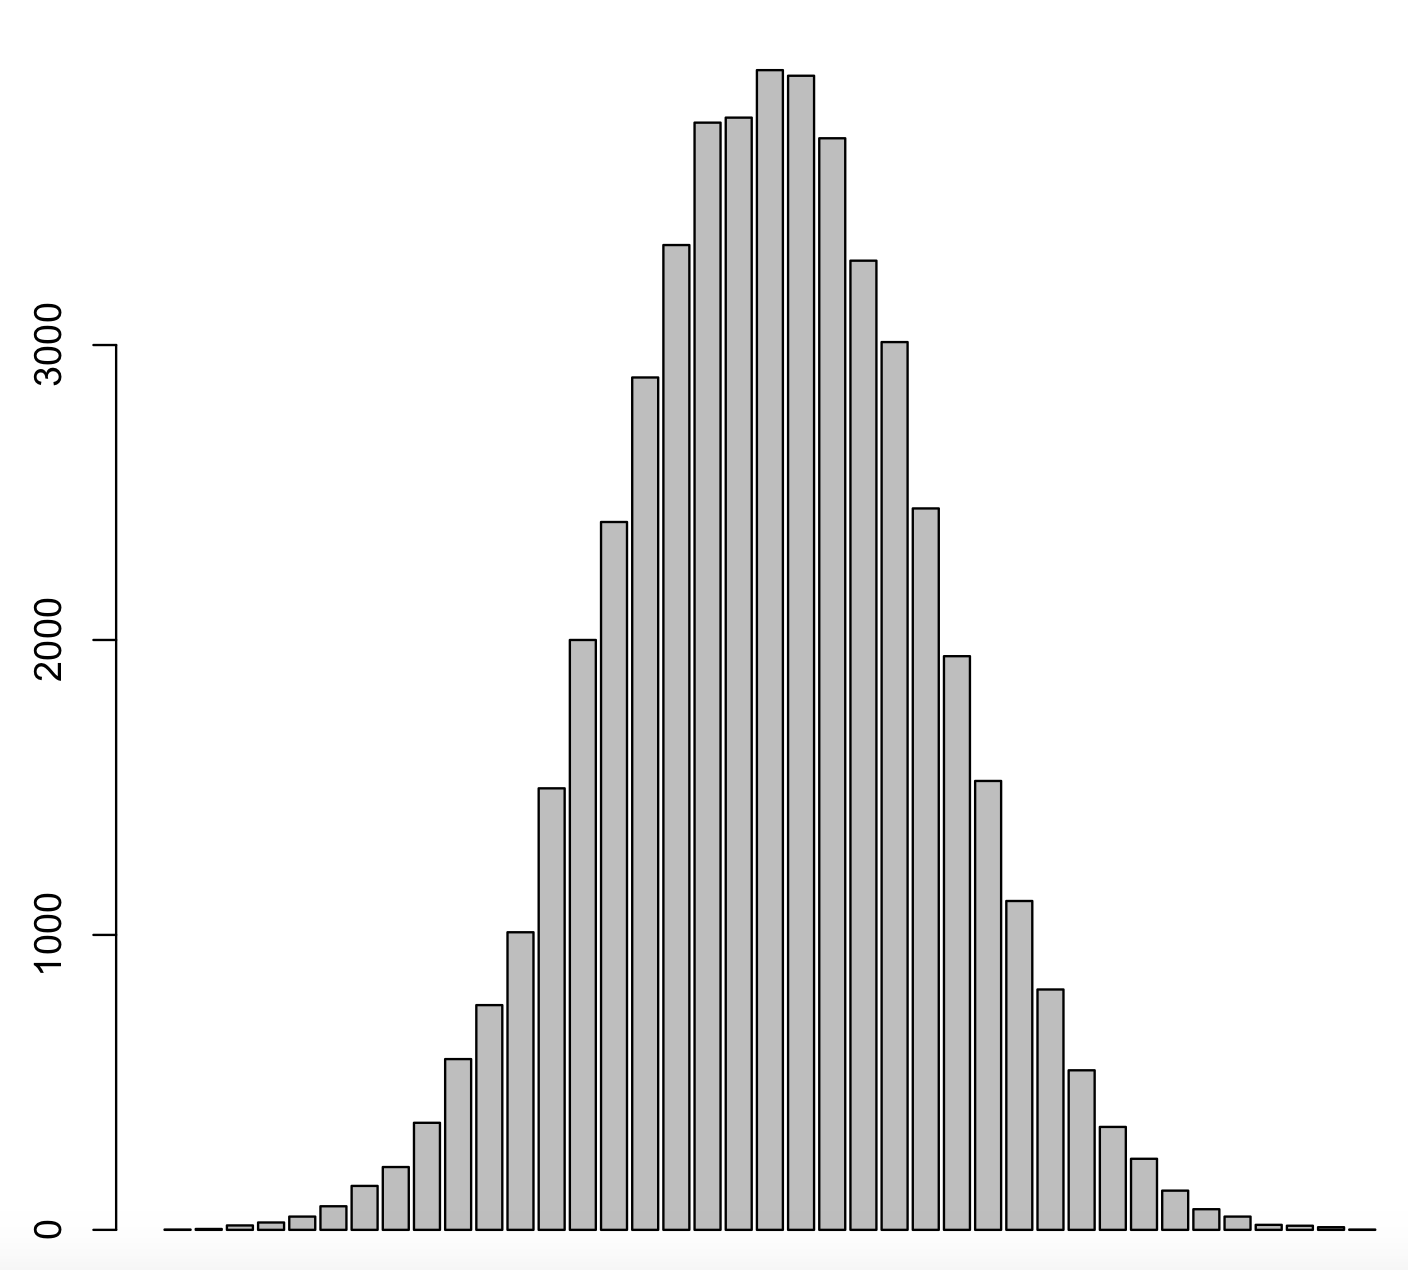
\includegraphics[width=0.5\textwidth]{figures/NormalDist.png}
    \caption{
      The result of \textit{barplot( table( rbinom(50000, 100, .5) ) )}}It looks exactly like a normal distribution.
    \label{fig:example_figure}
  \end{center}
\end{figure}


\subsection{Split Apply Combine Paradigm}

This paradigm entails loading all your data into memory. 
\begin{itemize}
	\item Split: Arrange observations into groups of interest (individual’s preferences/observations)
    \item Apply: Compute distributions/statistics
    \item Combine: Collect observations across groups
    \item Complexity: Time: 2N, N to split into groups, N to run distribution calculations, Space: 2N, copying grouped data to another place 
\end{itemize}
Note: If all we want is a running mean, and we know that before we get our data, then we can just use the running mean algorithm on the stream of data as we see it. Split/Apply/Combine allows us to do more with the data

Things to look out for with Split/Apply/Combine:
\begin{itemize}
	\item If, for example we're calculating the variance: $\frac{1}{N}\Sigma(x_i - \bar{x})^2$ 
    \item Note that the formula can be simplified to $\frac{1}{N}\Sigma({x_i}^2 - 2\bar{x}x_i + \bar{x}^2)$
    \item But even with the simplified expression, we have a squared term which can lead to significant problems if the number is a high value float (with a mean of $10^6$ the squared term becomes $10^12$ which can lead to overflows
    \item Another note: The median is simply the middle number in the distribution, but it is computationally infeasible to calculate the median in streaming data without storing all values.
\end{itemize}

\newpage

\textbf{Algorithm Shell for Split/Apply/Combine:}

\begin{algorithmic}
	\For{ each observation as (group, value)}:
		\State place value in bucket for corresponding group
    \EndFor
    \For{ each group }:
    	\State apply function over values in group
        \State output group and result
	\EndFor
\end{algorithmic}

This shell is useful when we are calculating within group statistics when we have required memory.


\subsection{The Long Tail}
The long tail is a statistical phenomenon where there is a small set of super popular things, followed by a very large set of moderately popular/unpopular things.\\
The long tail is often given as a reason why Netflix beat Blockbuster (even though in the early early days Netflix would have to mail you the movie when you would be able to just go drive to a Blockbuster).\\
Sampling on distributions with long tails is dangerous because its hard to model the tail drop off, so the distribution can easily be misrepresented.
\vspace{5mm}

\noindent \textbf{Algorithm for dealing with long tail streaming data:}
\begin{algorithmic}
	\For{ each observation as (group, value)}:
		\If {new group:}
        	Initialize result
        \EndIf
        \State Update result for corresponding group as function of existing result and current value
    \EndFor
    \For{ each group }:
    	\State apply function over values in group
        \State output group and result
	\EndFor
\end{algorithmic}
Though this algorithm seems really similar to what we've already seen, its really good for computing a subset of within group statistics like min, max, mean, variance with little memory usage.\newline
\textbf{Netflix Example:}
everyone likes the top 20 most popular movies, but we all also have weird esoteric tastes that are hard to service (at places like Blockbuster). For Blockbuster with physical locations it was easy to keep like 5000 most popular movies, but then our individual tastes get put aside for what's popular.

Perhaps we can use Split/Apply Combine here as well.\newline
\textbf{Pseudocode for Algorithm:}
\begin{algorithmic}
    
    \Function{Group By ID}{Dataset} \EndFunction
    
    \For {each Group in Dataset}:
    	\Function{Sort by Popularity}{Group}
        \EndFunction
	\EndFor 

    \For {each Group in Dataset}:
    	\Function{Cumulative Sum}{Group, Size of Data Set}
        \EndFunction
	\EndFor

\end{algorithmic}
Assume we have just grouped by ID
\newline
\newline
\begin{tabular}{l*{6}{c}r}
Movie ID          & Number of users wanting to watch & Cumulative percentage breakdown \\
\hline
Jurassic Park & 100 & 40.98 \%   \\
The Return of the King & 201 &  82.37 \% \\
Dances with Wolves    & 43 & 17.62 \%   \\
\end{tabular}

\begin{figure}[ht]
  \begin{center}
    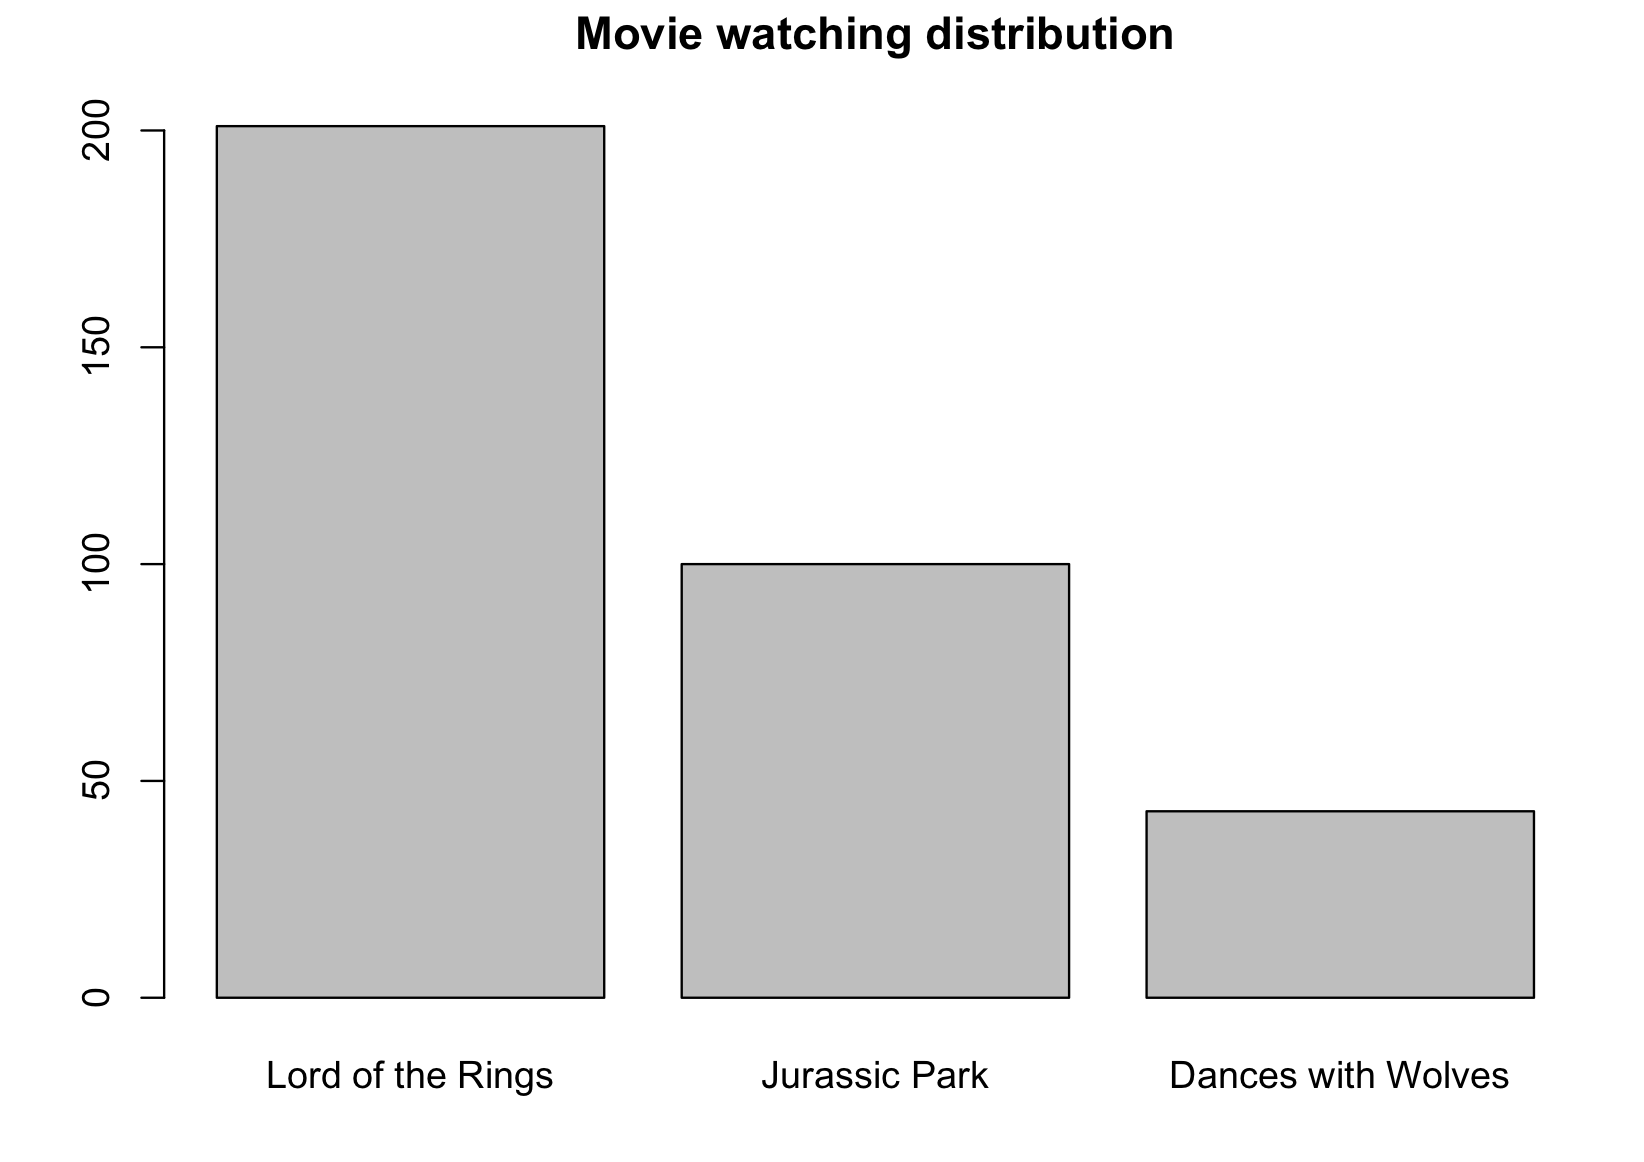
\includegraphics[width=0.5\textwidth]{figures/MovieDistribution.png}
    \caption{
      The result of graphing the cumulative movie preferences of all 344 users. Note how the distribution quickly tapers off at the end.}
    \label{fig:MovieDistribution}
  \end{center}
\end{figure}





\pagebreak
\textbf{Handy chart for performing group-by functions on Pregrouped data:}

\begin{tabular}{l*{6}{c}r}
Memory        & Scenario & Distributions & Statistics \\
\hline
N & Small dataset & Yes & General   \\
V*G   & Small Distributions &  Yes & General \\
G     & Small \# groups & No & Combinable   \\
V     & Small \# outcomes & Yes & General   \\
1     & Large \# both & No & Combinable   \\
\end{tabular}

\textbf{Legend:}
\begin{itemize}
	\item N = total number of observations
    \item G = number of distinct groups
    \item V = largest number of distinct vales within group
\end{itemize}

\subsection{Practical Shell Stuff:}

\begin{itemize}
	\item \textbf{man}: gives users guide to the next function argument
	\item \textbf{ls}: lists directory contents, optional arguments include details of ownership/execute privileges
    \begin{itemize}
    	\item ls -a -l: these options allow you to see all files in a listed format
        \item ls -alh: file sizes
        \item ls -l *.sh: all .sh files
    \end{itemize}
	\item \textbf{bash}: Bourne Again Shell, interactive programming environment where programs/executables can be run and directories can be navigated
	\item \textbf{more}:  allows for quick examination of a file in the shell (so without using a text editor to walk through the file)
	\item \textbf{less}: Allows for quick exploration of a file like more but also allows one to go 'backwards' or to previous content in file
    \begin{itemize}
    	\item double quotes in the shell: allows for expansion of variables from the shell
		\begin{itemize}
			\item all characters are treated the same except for \$ and ' which are expanded in shell
		\end{itemize}
        \item single quotes: expression is strictly, literally, interpreted
    \end{itemize}
\end{itemize}











